\documentclass{article}

\usepackage{booktabs}
\usepackage{tabularx}
\usepackage{graphicx}

\title{Development Plan\\\progname}

\author{\authname}
\setlength\parindent{0pt}
\date{}

%% Comments

\usepackage{color}

\newif\ifcomments\commentstrue %displays comments
%\newif\ifcomments\commentsfalse %so that comments do not display

\ifcomments
\newcommand{\authornote}[3]{\textcolor{#1}{[#3 ---#2]}}
\newcommand{\todo}[1]{\textcolor{red}{[TODO: #1]}}
\else
\newcommand{\authornote}[3]{}
\newcommand{\todo}[1]{}
\fi

\newcommand{\wss}[1]{\authornote{blue}{SS}{#1}} 
\newcommand{\plt}[1]{\authornote{magenta}{TPLT}{#1}} %For explanation of the template
\newcommand{\an}[1]{\authornote{cyan}{Author}{#1}}

%% Common Parts

\newcommand{\progname}{ProgName} % PUT YOUR PROGRAM NAME HERE
\newcommand{\authname}{Team \#, Team Name
\\ Student 1 name and macid
\\ Student 2 name and macid
\\ Student 3 name and macid
\\ Student 4 name and macid} % AUTHOR NAMES                  

\usepackage{hyperref}
    \hypersetup{colorlinks=true, linkcolor=blue, citecolor=blue, filecolor=blue,
                urlcolor=blue, unicode=false}
    \urlstyle{same}
                                


\begin{document}

\begin{table}[hp]
\caption{Revision History} \label{TblRevisionHistory}
\begin{tabularx}{\textwidth}{llX}
\toprule
\textbf{Date} & \textbf{Developer(s)} & \textbf{Change}\\
\midrule
September 26 & N/A & Initial documentation\\
\bottomrule
\end{tabularx}
\end{table}

\newpage

\maketitle

\wss{Put your introductory blurb here.}

\section{Team Meeting Plan}
Weekly meetings to be held every Saturday at 8:00PM, and additional meetings to be planned as needed. Any meetings requiring the attendance of supervisor will have to be planned based on Dr. Macedo's availability each time. In cases of team members' absence, each absent team members are expected to bring forward their discussion topics prior to the scheduled meeting time, and review the meeting notes posted in the Discord server. Team leaders are expected to write down meeting notes for each meeting, regardless of the number of participating members.\\

\section{Team Communication Plan}
All main communication channel will be done through the Discord server, including all meetings. Secondary communication will be through Facebook group chat if necessary.\\

The following is a screen shot of this team's Discord server:\\
\begin{center}
    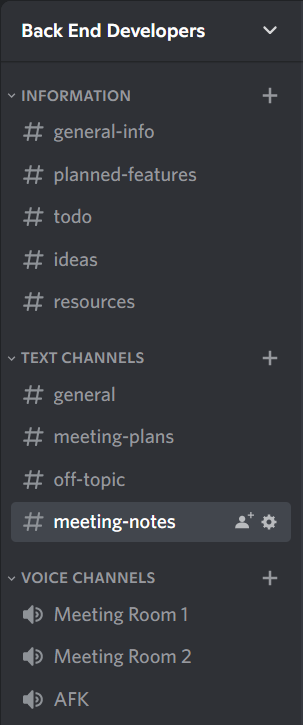
\includegraphics{DiscordServer}
\end{center}

\section{Team Member Roles}
The team will have 2 team leaders (co-leaders), Jonathan Hai and Jessica Bae will take this role. The responsibilities of team leaders are to organize meetings, record meeting notes, assign specific tasks to all team members, overlook deliverable deadlines, keep track of overall team project progress, and communicate with the TA, the professor, and the supervisor.\\

The team will also have a Github leader, responsible for managing all technical Github merge requests and approving them. Labeeb Zaker will take on this role.\\

The task of eviewing rubrics, and each subcomponents of the project will not be assigned to any specific member. These tasks are to be allocated to different members each time, to be decided as needed.\\

\section{Workflow Plan}
For any documentation, team members are not required to put in a merge request. For any technical commits, everyone is required to put in a merge request for the Github leader to review and approve. Trello will be used for project management purposes (non-technical tasks) and Github issue tracker will be used for technical tasks.\\

\section{Proof of Concept Demonstration Plan}

What is the main risk, or risks, for the success of your project?  What will you
demonstrate during your proof of concept demonstration to convince yourself that
you will be able to overcome this risk?

\section{Technology}

\begin{itemize}
\item Specific programming language
\item Specific linter tool (if appropriate)
\item Specific unit testing framework
\item Investigation of code coverage measuring tools
\item Specific plans for Continuous Integration (CI), or an explanation that CI
  is not being done
\item Specific performance measuring tools (like Valgrind), if
  appropriate
\item Libraries you will likely be using?
\item Tools you will likely be using?
\end{itemize}

\section{Coding Standard}

\section{Project Scheduling}

Firstly, a Master Project Schedule will be made with a list of all the deadlines, deliverables and Project Implementation tasks. Work will be done based on weekly sprints where tasks will be assigned to each member along with an estimated number of days needed to finish the task. This number is evaluated based on relative complexity of each task.\\

Secondly, the team imposed deadline for all tasks are \textbf{two} days before the due date of the deliverable. On this day, the team will conduct a review of all the work done by the members and provide any feedback. The last day before the due date is reserved for making any final changes and small revisions. Moreover, the team will check the completed deliverable with the marking rubric.\\

Finally, every two weeks, a design overhaul will be conducted wherein the team will go through the previous parts of the project and update it with any changes made as a result of the current iteration of the project.\\







\end{document}